% Carried over verbatim from monograph/main.tex (Study 1 record, 13 Sep 2026).
\chapter{Cx22 segmentation rescore}\label{s1:ch:ch11_cx22_segmentation_rescore}

\section{Why add a second task and dataset?}

Classification alone could leave two alternative explanations: perhaps the phenomenon is specific to SIPaKMeD, or perhaps it is specific to assigning a single label to a crop. Cx22 offers a different hierarchy and two pixel-level tasks. It therefore tests whether the split logic transfers to semantic and instance segmentation without pretending that its official split is the same estimand as the pooled stress test.

The pooled analysis treats all 1,320 released generated regions as the observation pool and the 514 CCEDD sources as parents. The protocol{OFFICIAL} arm uses only Cx22-Multi-Train (400 observations) and Cx22-Multi-Test (100 observations). These official train and test source-parent sets are disjoint. Pair is not added to the official test comparison: 55 of its source parents overlap Multi-Test and 233 overlap Multi-Train, with Jaccard similarities 0.126 and 0.475 respectively. Pooling and re-splitting is thus a downstream-reuse stress test, not an accusation that the authors' official Multi split is flawed.

\section{Targets and models}

The semantic target has two independent binary channels: cytoplasm and nucleus. Five encoder--decoder families are re-run: U-Net~\cite{ronneberger2015unet}, U-Net++~\cite{zhou2020unetplusplus}, DeepLabV3+~\cite{chen2018deeplabv3plus}, FPN~\cite{lin2017fpn}, and MAnet~\cite{fan2020manet}. ResNet-34 is the encoder except for DeepLabV3+, which uses ResNet-50. All encoders start from ImageNet weights. The output activation is not embedded in the network; logits are passed through sigmoid in the loss and evaluation code.

For image $i$, channel $c$, prediction probability $p_{icu}$, and binary target $y_{icu}$ at pixel $u$, the training objective is
\begin{align}
\mathcal L_{\mathrm{semantic}}
&=\mathcal L_{\mathrm{BCE}}+\mathcal L_{\mathrm{softDice}},\\
\mathcal L_{\mathrm{softDice}}
&=1-\frac{1}{2N}\sum_{i,c}
\frac{2\sum_u p_{icu}y_{icu}+1}
{\sum_u p_{icu}+\sum_u y_{icu}+1}.
\end{align}

The instance task uses Mask R-CNN with a ResNet-50 FPN backbone and its torchvision V2 implementation~\cite{he2017maskrcnn}. The classification and mask heads are replaced for one foreground category plus background. Ground-truth cytoplasm instances are reconstructed from the released MATLAB label structure before resizing. Empty instances after resizing are rejected rather than silently retained.

\section{Deterministic input construction}

All images and masks are resized to $256\times256$; RGB images use antialiased interpolation, while masks use nearest-neighbor interpolation. Training augmentation is determined by a SHA-256 digest of seed, epoch, and crop ID. Digest bits choose horizontal flip, vertical flip, and one of four right-angle rotations. This produces per-epoch augmentation without relying on worker scheduling order. Images are ImageNet-normalized; masks remain binary.

The original JPEGs and generated masks were packed into memory-mappable arrays, each named in a provenance manifest with SHA-256 hashes and a cache version. This was not a scientific transformation. It removed repeated JPEG/MATLAB/NFS decoding from the inner loop while making the exact input bytes auditable.

\begin{table}[H]
\centering
\caption{Cx22 segmentation execution settings.}
\label{s1:tab:cx22-hparams}
\begin{tabular}{lll}
\toprule
Item & Semantic & Instance \\
\midrule
Image size & $256\times256$ & $256\times256$ \\
Epochs & 30 & 30 \\
Batch size & 16 & 2 (test batch 1) \\
Optimizer & AdamW & AdamW \\
Learning rate & $10^{-4}$ fixed & $10^{-4}$ fixed \\
Weight decay & $10^{-4}$ & $10^{-4}$ \\
Precision & FP16 except MAnet FP32 & FP16 \\
Endpoint schedule & every epoch; final retained & final epoch only \\
Checkpointing & every epoch & every 5 epochs \\
Seeds & 17, 29, 43, 71, 101 & 17, 29, 43, 71, 101 \\
Hardware & \multicolumn{2}{l}{NVIDIA RTX A6000; at most three concurrent GPU jobs} \\
\bottomrule
\end{tabular}
\end{table}

\section{Semantic metrics}

Probabilities are thresholded at 0.5. For predicted set $A$ and target set $B$,
\begin{equation}
\operatorname{Dice}(A,B)=\frac{2|A\cap B|}{|A|+|B|},\qquad
\operatorname{IoU}(A,B)=\frac{|A\cap B|}{|A\cup B|}.
\end{equation}
The primary semantic value first averages cytoplasm and nucleus Dice within each image, then averages over test images. This prevents a large cytoplasm region from numerically drowning the smaller nucleus. Channel-specific Dice and IoU are retained as diagnostic endpoints.

\section{Instance matching metric}

Predictions with object score below 0.5 are discarded. Let $D_{jk}$ be Dice between predicted instance $j$ and ground-truth instance $k$. The Hungarian assignment~\cite{kuhn1955hungarian} maximizes
\begin{equation}
\max_{\pi}\sum_{(j,k)\in\pi}D_{jk}
\end{equation}
subject to one-to-one matching. Every unmatched ground-truth instance receives Dice and IoU zero. The primary image value is the mean over that image's ground-truth instances; images are then averaged. Recall@0.70 is the fraction of ground-truth instances whose matched Dice is at least 0.70. This endpoint penalizes missed cells and does not allow an image with many easy instances to dominate the result.

\begin{lstlisting}[style=cyto,caption={Exact logic of the matched-instance endpoint.},label={lst:instance-metric}]
keep predictions with confidence >= 0.50
threshold predicted and target masks at 0.50
compute all predicted-by-target Dice values on the GPU
solve maximum-weight one-to-one assignment
write matched Dice into a zero vector of length n_targets
average the vector within the image
average image means over the test set
\end{lstlisting}

\section{Semantic results}

\begin{table}[H]
\centering
\caption{Cx22 semantic macro-Dice (\%), mean $\pm$ sample SD over five seeds. The official column uses a different 400/100 sample and is descriptive, not a paired protocol contrast.}
\label{s1:tab:cx22-semantic}
\small
\begin{tabular}{lrrrrr}
\toprule
Model & \protocol{P1} & \protocol{P1$'$} & \protocol{P2} & \protocol{P3} & \protocol{OFFICIAL} \\
\midrule
DeepLabV3+ & 88.90$\pm$0.45 & 88.84$\pm$0.45 & 88.64$\pm$0.34 & 88.10$\pm$0.38 & 82.96$\pm$1.54 \\
FPN & 88.90$\pm$0.43 & 88.97$\pm$0.55 & 88.89$\pm$0.48 & 88.33$\pm$0.30 & 84.43$\pm$0.33 \\
MAnet & 90.03$\pm$0.60 & 90.07$\pm$0.63 & 89.97$\pm$0.45 & 89.63$\pm$0.21 & 85.50$\pm$1.41 \\
U-Net & 90.29$\pm$0.48 & 90.32$\pm$0.52 & 89.99$\pm$0.52 & 89.77$\pm$0.16 & 85.64$\pm$0.58 \\
U-Net++ & 90.56$\pm$0.51 & 90.58$\pm$0.54 & 90.38$\pm$0.35 & 90.05$\pm$0.21 & 87.30$\pm$1.13 \\
\bottomrule
\end{tabular}
\end{table}

\begin{figure}[H]
\centering
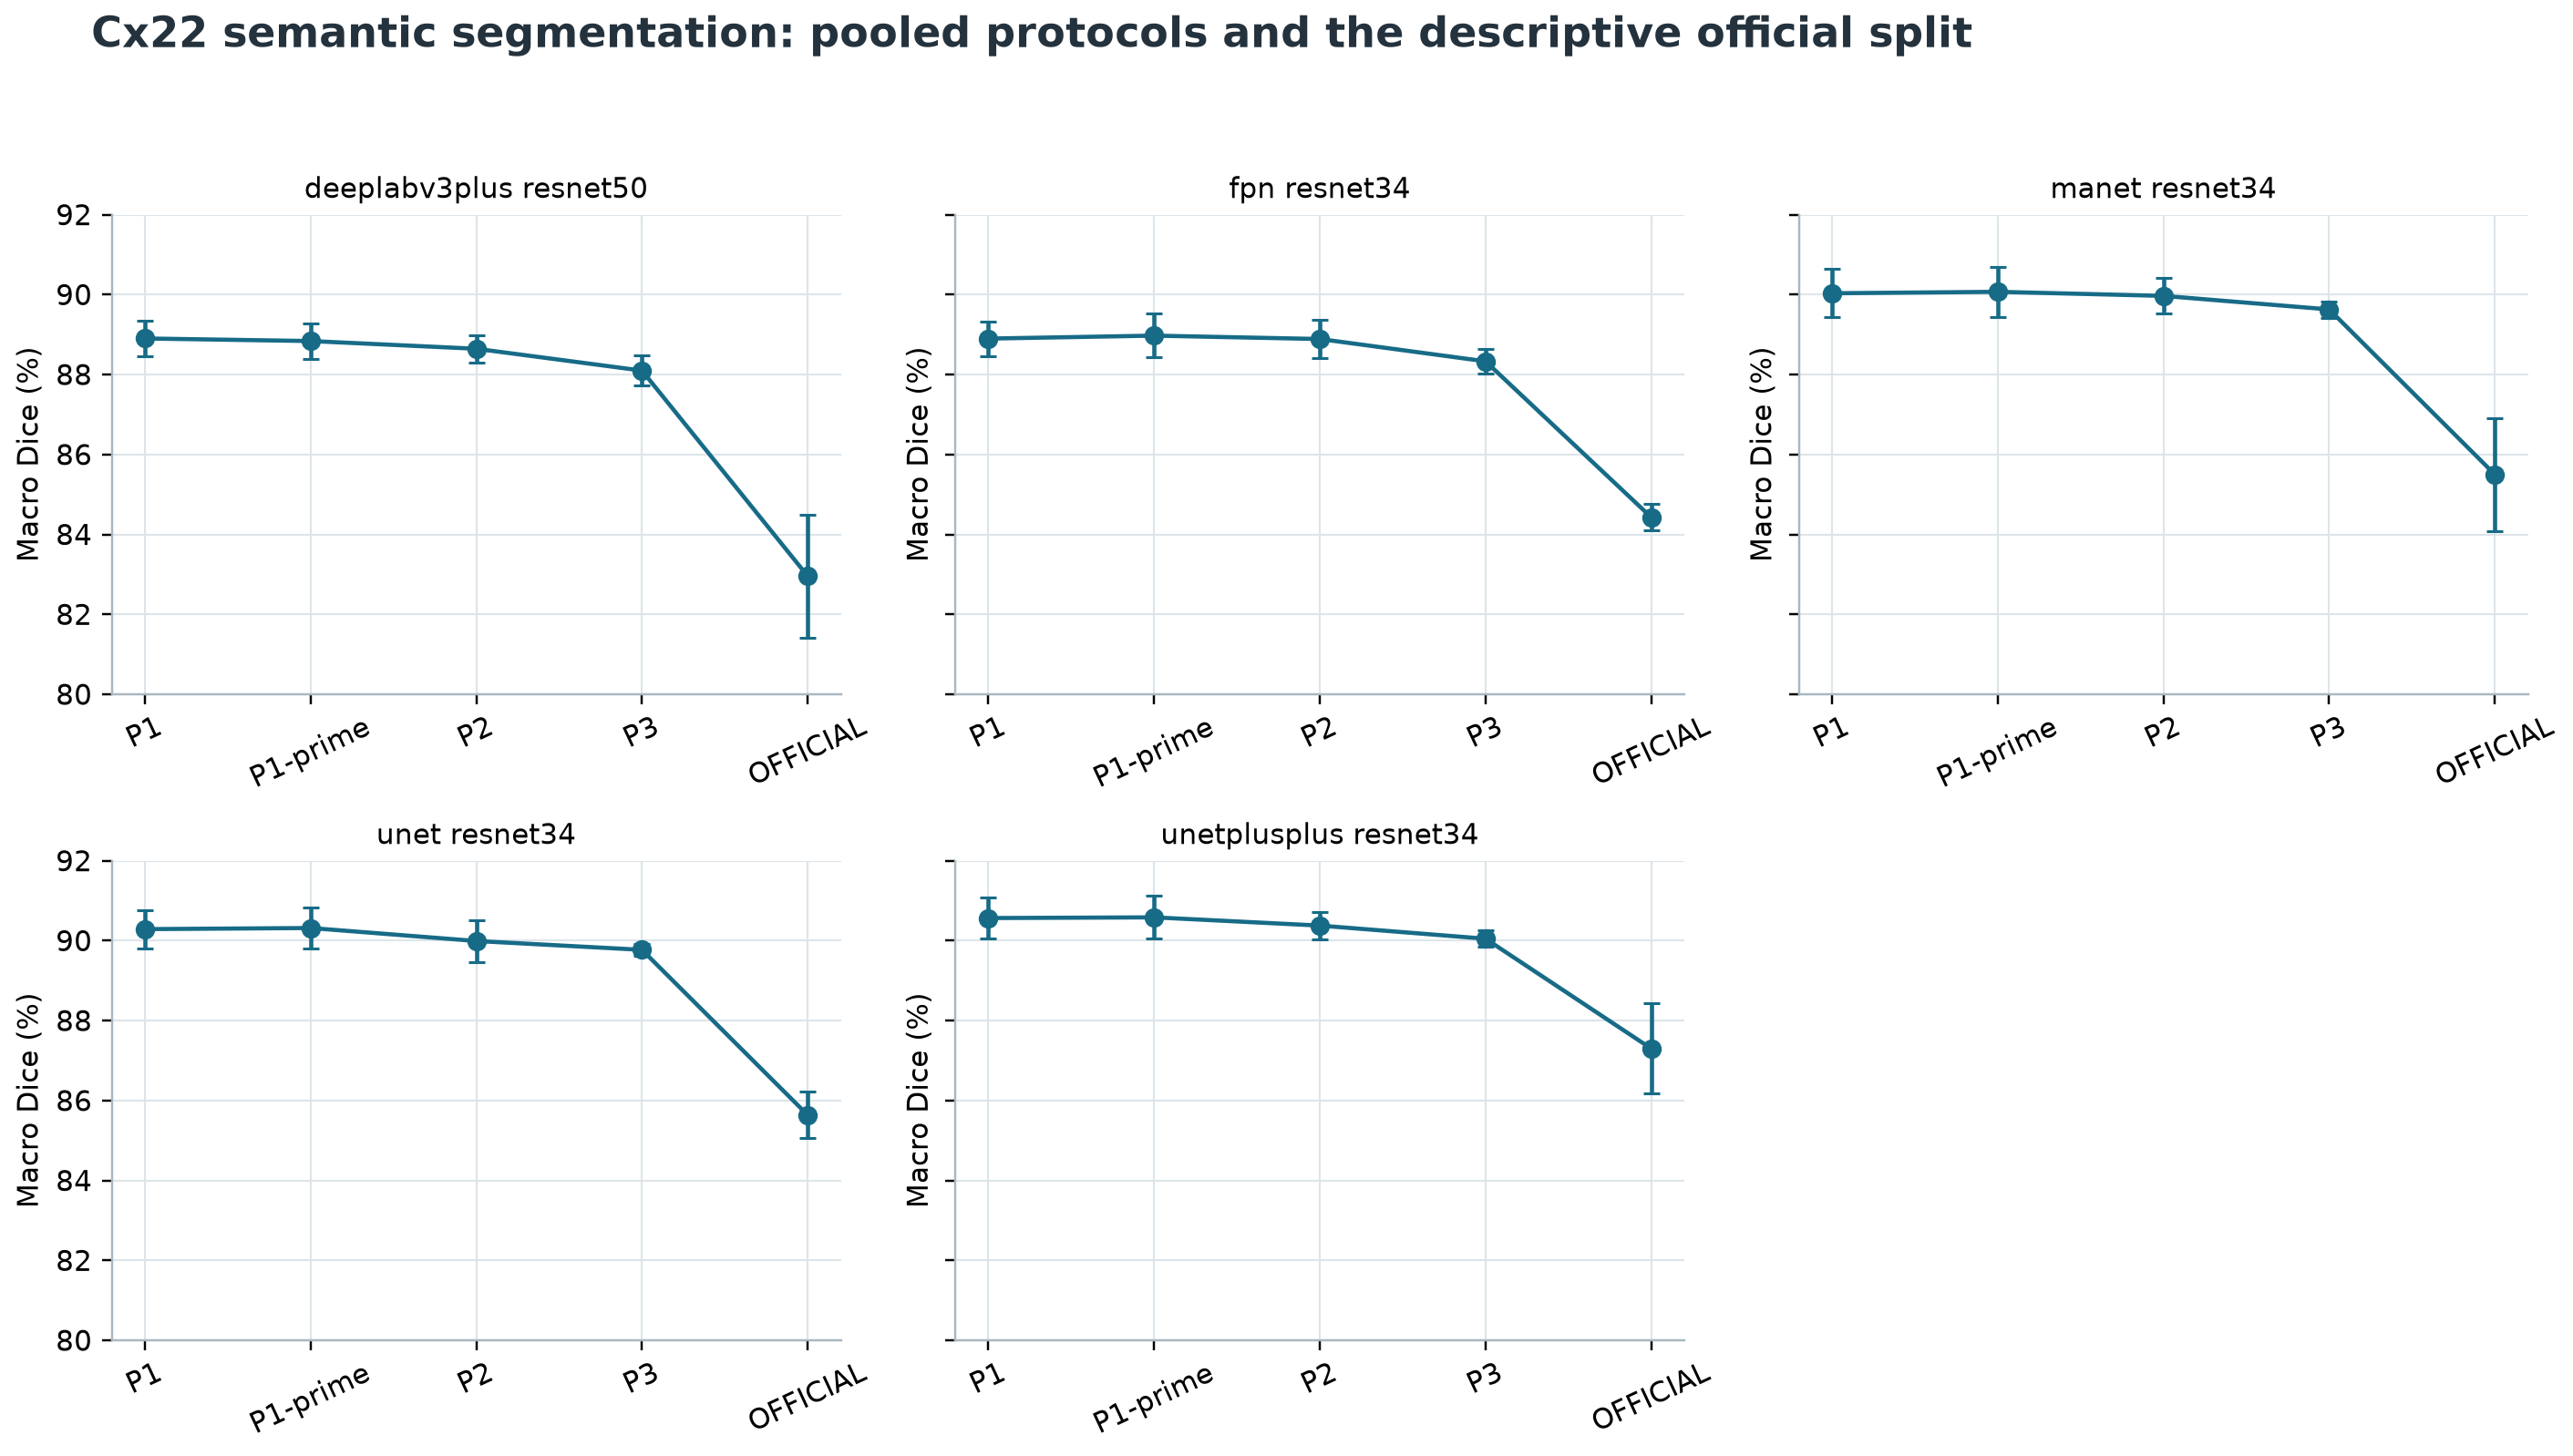
\includegraphics[width=\textwidth]{cx22_semantic_scores.png}
\caption{Cx22 semantic macro-Dice by architecture and protocol. The official arm is visually separated because it is not a same-observation contrast.}
\label{s1:fig:cx22-semantic}
\end{figure}

\begin{figure}[H]
\centering
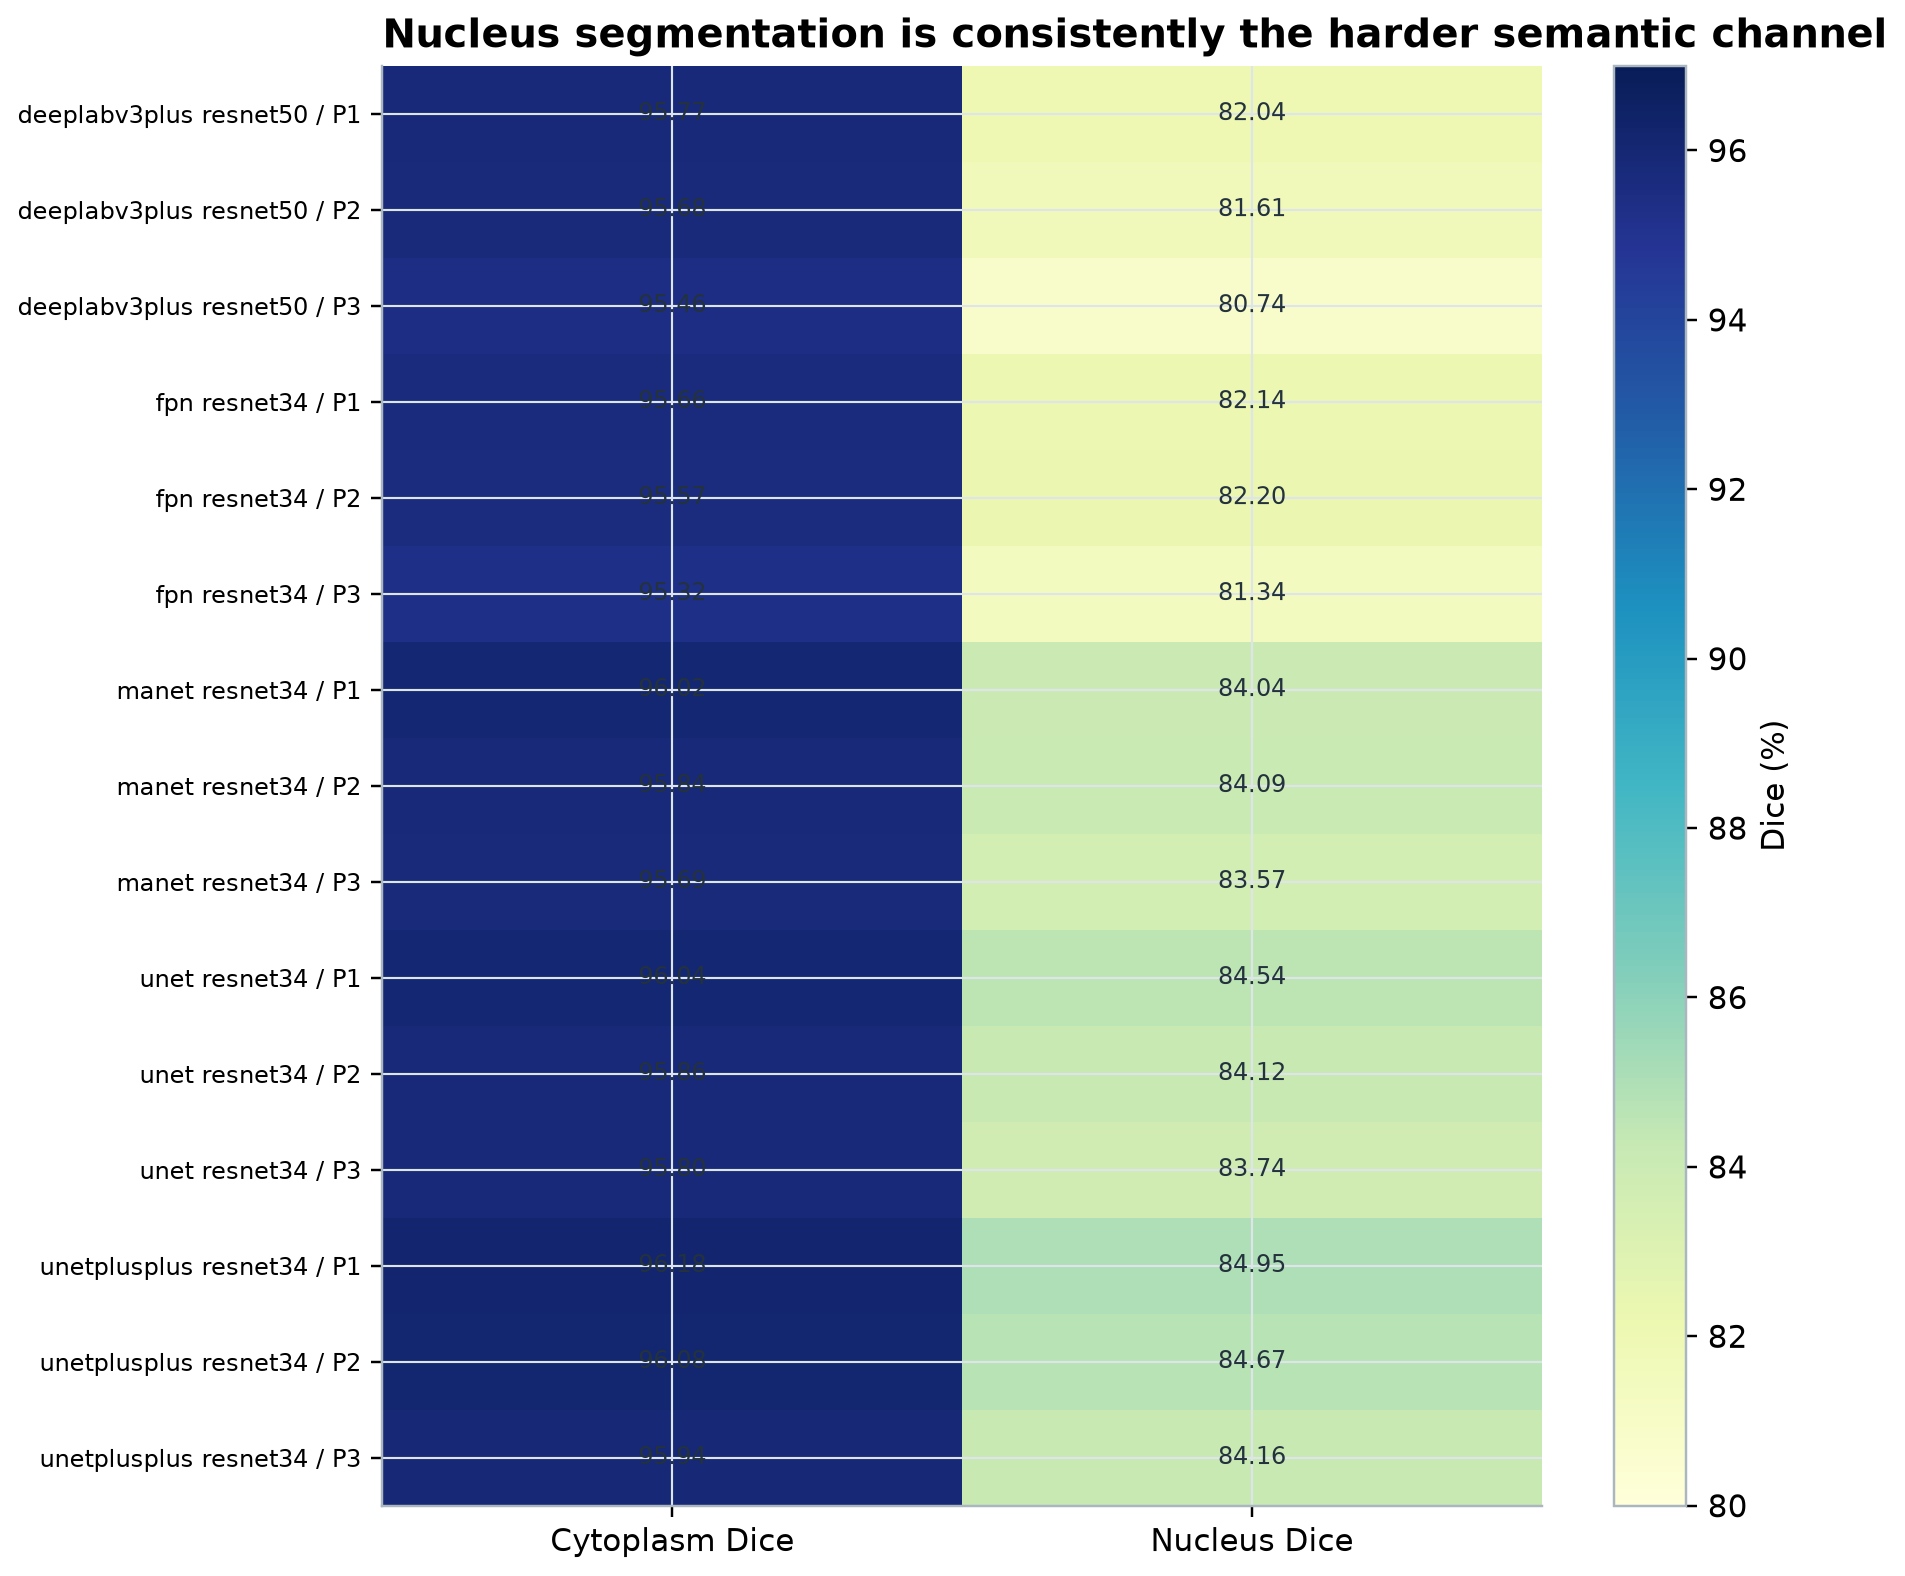
\includegraphics[width=\textwidth]{cx22_channel_heatmap.png}
\caption{Channel-level Dice makes the central difficulty visible: nuclei are consistently harder than cytoplasm. This is the segmentation analogue of a confusion-matrix diagnostic and uses retained aggregate channel measurements, not invented pixel predictions.}
\label{s1:fig:cx22-channels}
\end{figure}

U-Net++ is best in every pooled protocol and on the official Multi arm. The channel breakdown explains the lower official macro score: across models, cytoplasm Dice is roughly 94--95\% while nucleus Dice is roughly 72--79\%. Nuclei are smaller, so a fixed boundary displacement consumes a larger fraction of their area; faint staining and overlap also make the boundary less stable. This is a checkable data property visible in the released masks rather than a generic explanation added after the fact.

\section{Instance results}

\begin{table}[H]
\centering
\caption{Cx22 matched-instance Dice (\%), mean $\pm$ sample SD over five seeds.}
\label{s1:tab:cx22-instance}
\small
\begin{tabular}{lrrrrr}
\toprule
Model & \protocol{P1} & \protocol{P1$'$} & \protocol{P2} & \protocol{P3} & \protocol{OFFICIAL} \\
\midrule
Mask R-CNN & 92.10$\pm$0.52 & 92.05$\pm$0.52 & 91.59$\pm$0.42 & 91.11$\pm$1.09 & 92.29$\pm$0.32 \\
Mask R-CNN V2 & 91.99$\pm$0.57 & 91.95$\pm$0.58 & 91.36$\pm$0.82 & 90.60$\pm$0.52 & 92.18$\pm$0.71 \\
\bottomrule
\end{tabular}
\end{table}

\begin{figure}[H]
\centering
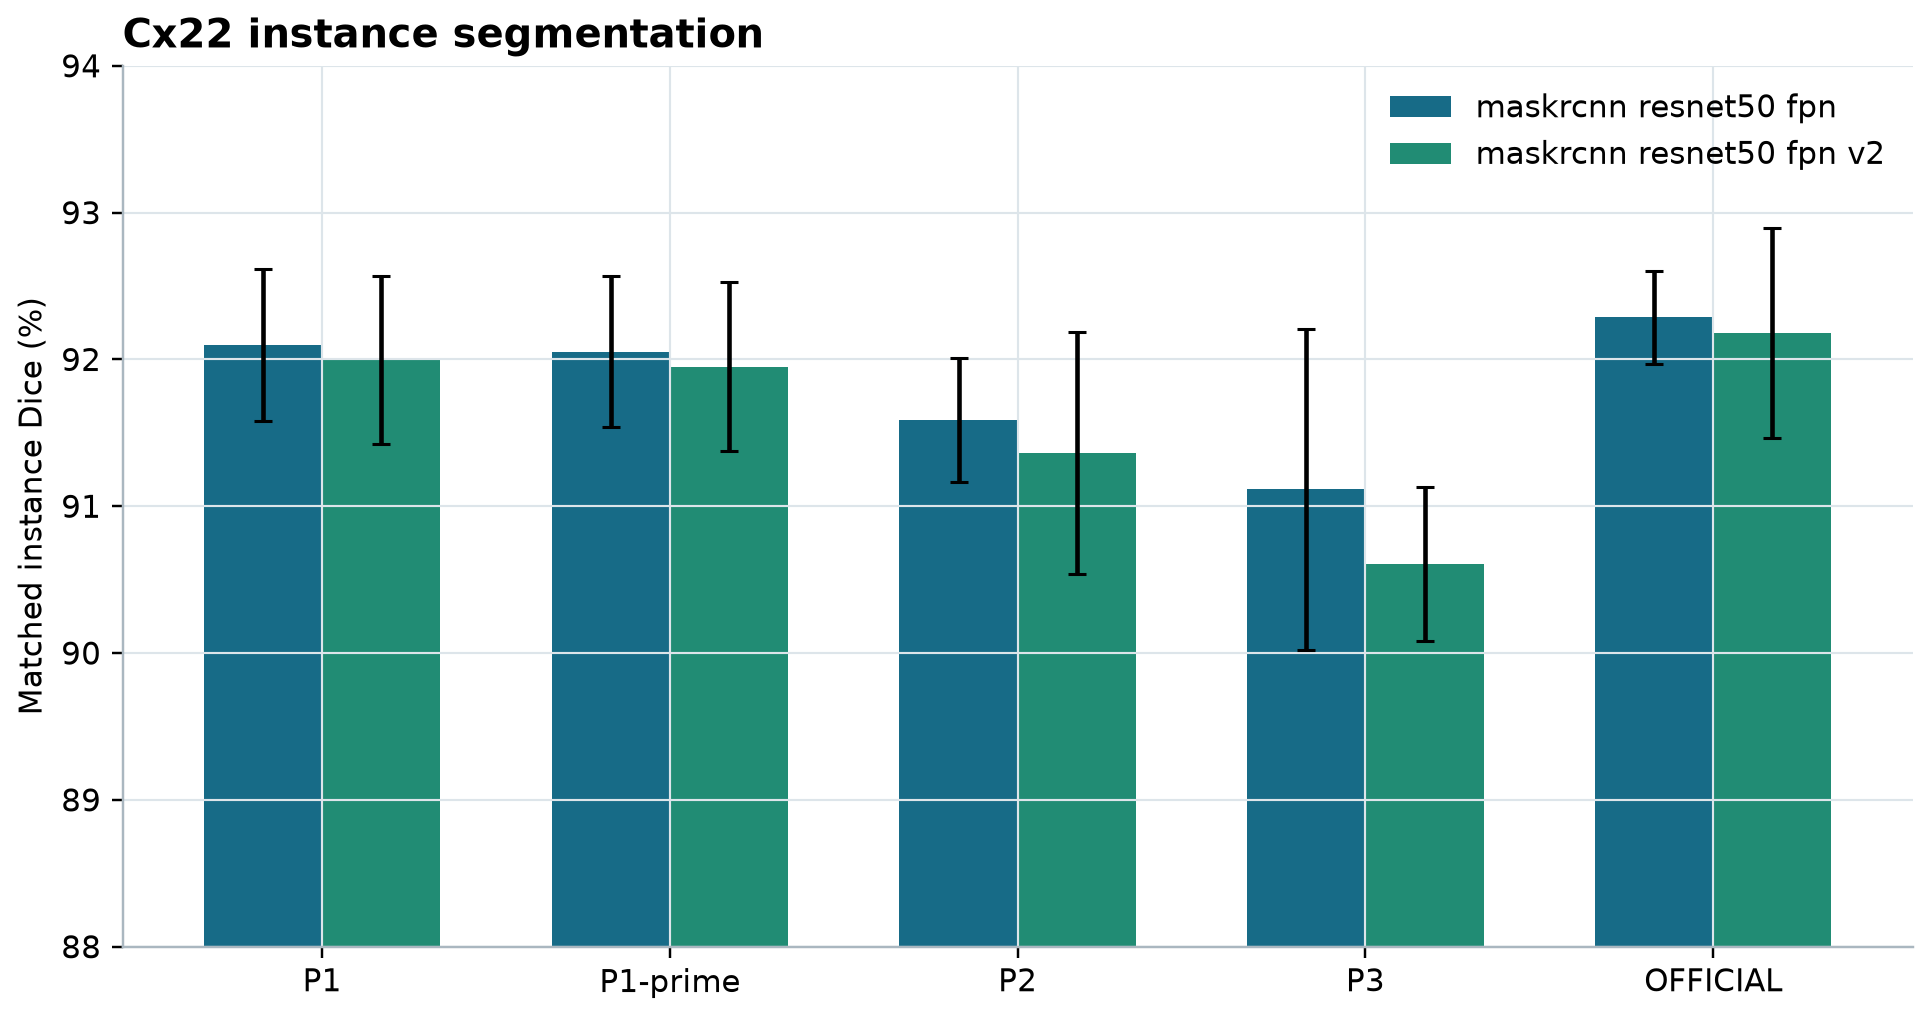
\includegraphics[width=\textwidth]{cx22_instance_scores.png}
\caption{Cx22 matched-instance Dice. Both Mask R-CNN variants follow the complete registered \protocol{P3}$\leq$\protocol{P2}$\leq$\protocol{P1} ordering.}
\label{s1:fig:cx22-instance}
\end{figure}

Unlike SIPaKMeD classification, all seven Cx22 architecture/task rows satisfy the registered ordering. The differences are still small: \protocol{P1}$-$\protocol{P2} is 0.01--0.30 percentage points for semantic models and 0.51--0.63 points for instance models.

\section{Inference and rank stability}

\begin{table}[H]
\centering
\caption{Primary Cx22 \protocol{P1}$-$\protocol{P2} contrasts. Values are mean $\pm$ SD percentage points; $q$ is within the task-specific preregistered family. Effect is Cohen's $d_z$ except DeepLabV3+, whose non-normal seed differences trigger rank-biserial effect size.}
\label{s1:tab:cx22-primary}
\small
\begin{tabular}{llrrrr}
\toprule
Task & Model & Mean$\pm$SD & Raw $p$ & BH $q$ & Effect \\
\midrule
Semantic & DeepLabV3+ & 0.258$\pm$0.418 & 0.3125 & 0.8458 & 0.600$^{\dagger}$ \\
Semantic & FPN & 0.010$\pm$0.468 & 0.9625 & 0.9625 & 0.022 \\
Semantic & MAnet & 0.065$\pm$0.450 & 0.7612 & 0.8458 & 0.146 \\
Semantic & U-Net & 0.297$\pm$0.767 & 0.4353 & 0.8458 & 0.387 \\
Semantic & U-Net++ & 0.188$\pm$0.406 & 0.3582 & 0.8458 & 0.464 \\
Instance & Mask R-CNN & 0.509$\pm$0.581 & 0.1220 & 0.2440 & 0.875 \\
Instance & Mask R-CNN V2 & 0.630$\pm$1.204 & 0.3068 & 0.3116 & 0.523 \\
\bottomrule
\multicolumn{6}{l}{\footnotesize $^{\dagger}$rank-biserial correlation; all other effects are Cohen's $d_z$.}
\end{tabular}
\end{table}

\begin{figure}[H]
\centering
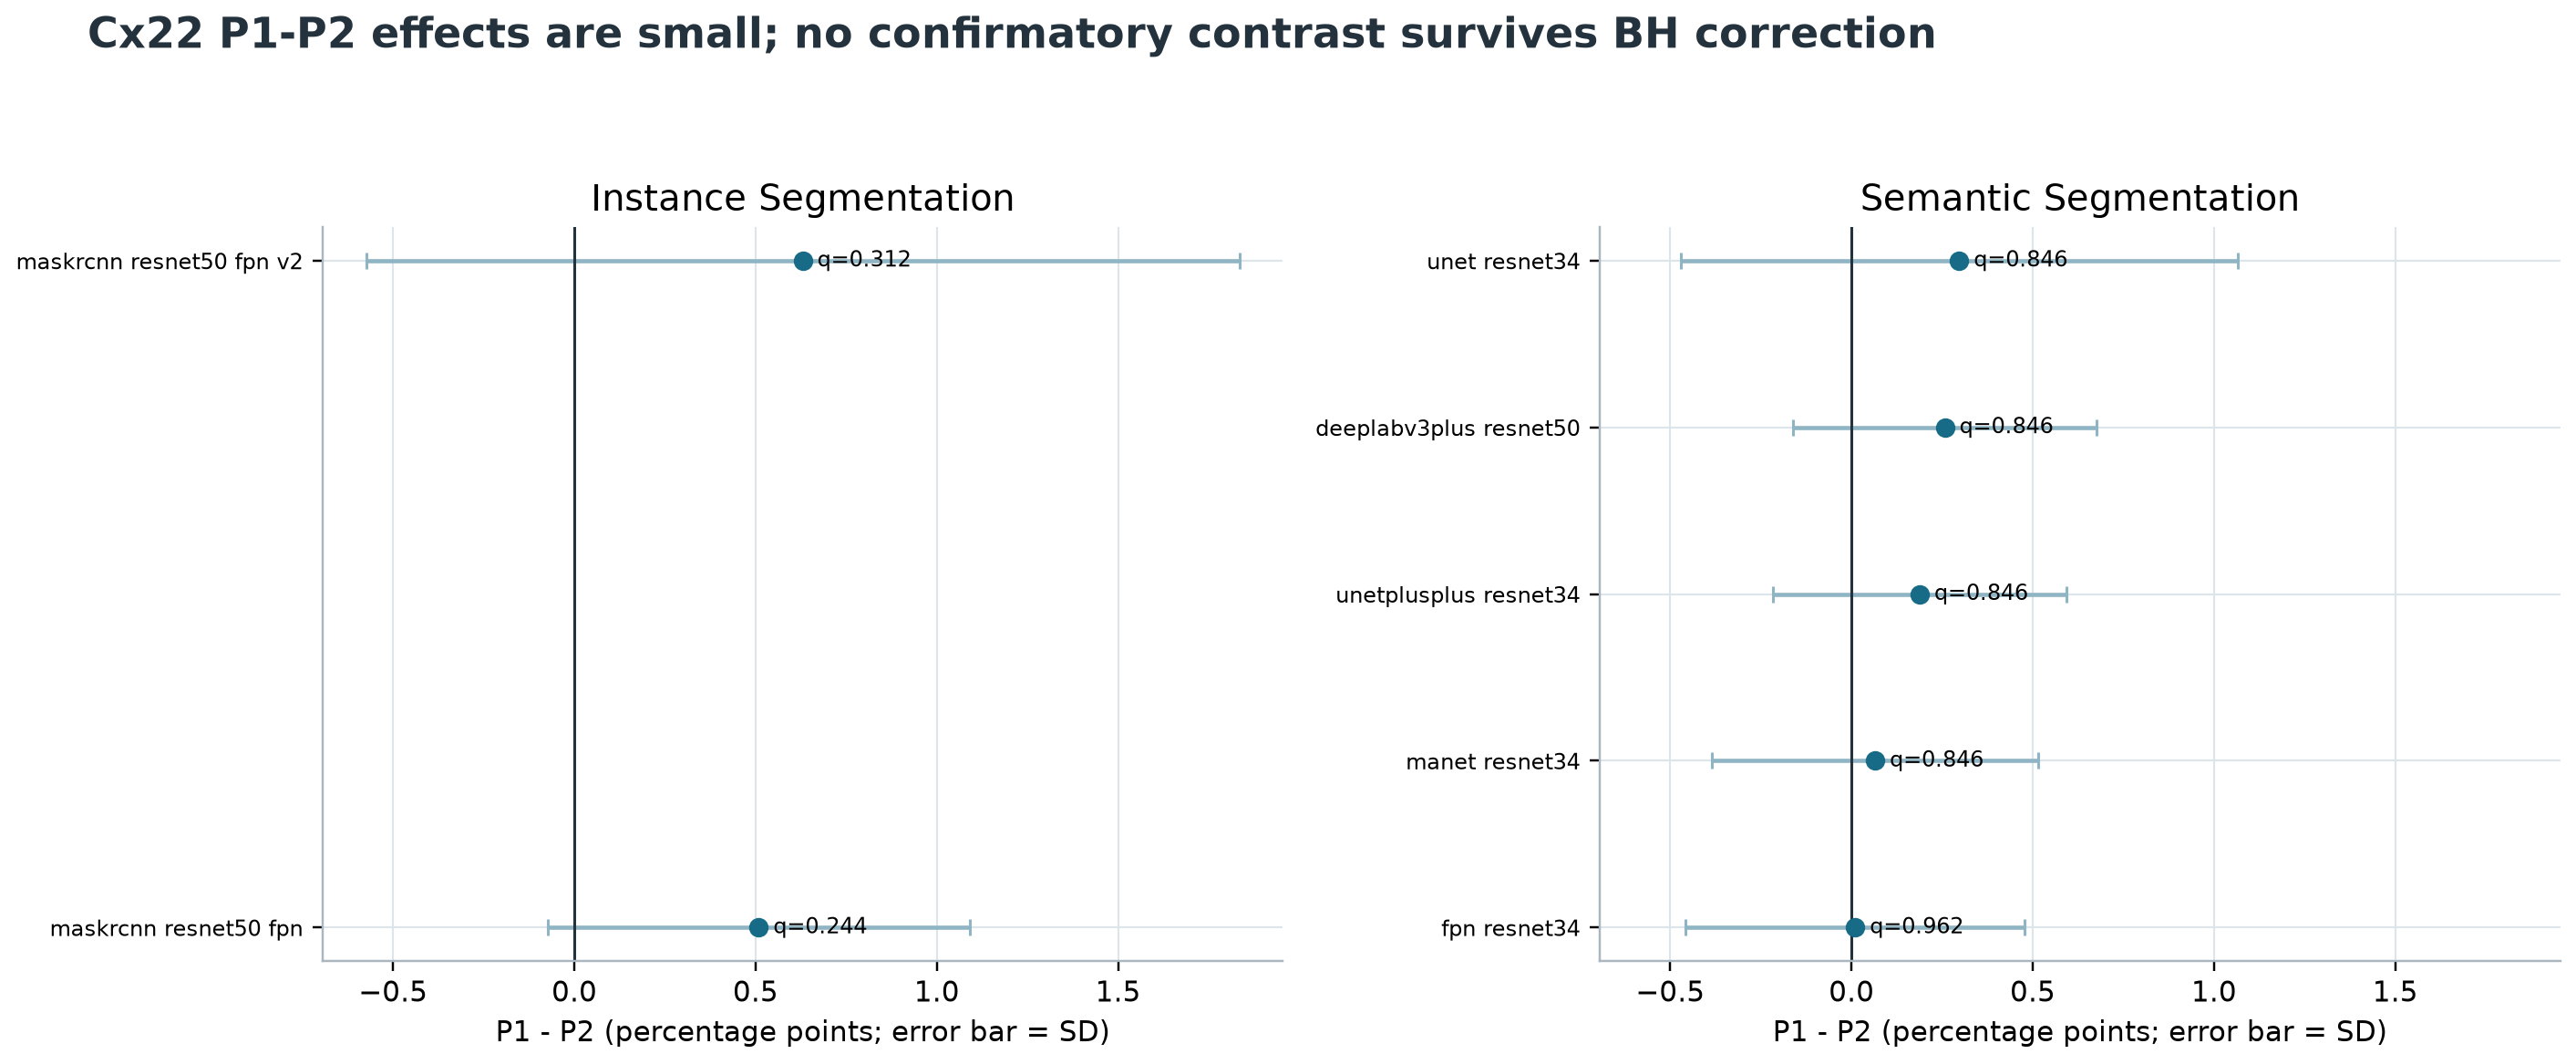
\includegraphics[width=\textwidth]{cx22_contrasts.png}
\caption{Cx22 paired contrast overview. Positive values favor the crop-level protocol. The plot separates point-estimate consistency from multiplicity-adjusted evidence.}
\label{s1:fig:cx22-contrasts}
\end{figure}

No primary Cx22 test survives BH correction. The size-matched \protocol{P1$'$}$-$\protocol{P2} Mask R-CNN contrast has raw $p=0.0377$, $d_z=1.368$, and $q=0.1508$; it is not promoted to a significant claim. In the explicitly secondary \protocol{P2}$-$\protocol{P3} family, FPN has raw $p=0.0226$ and $d_z=1.613$; it remains secondary and is not used to rescue the main conclusion.

Semantic model ranking is comparatively stable: Kendall's $\tau=0.8$ with bootstrap interval [0.6, 1.0], $p=0.0833$, and one of ten model pairs reordered. With only two instance models, $\tau=1.0$ but its bootstrap interval spans [$-1$,1], which is appropriately uninformative.

\section{Training failures, recovery, and runtime}

The first MAnet \protocol{P1}, seed-17 attempts produced non-finite losses at epochs 23 and 24 under FP16, despite dynamic loss scaling. Retaining an epoch-22 model or changing only that seed would have biased the matrix. The matrix stopped at 100 of 175 cells, the failure was amended in writing, and every MAnet cell was restarted in FP32 from its fixed seed. The corrected runs also set \artifact{CUBLAS_WORKSPACE_CONFIG=:4096:8} before any corrected MAnet or instance result existed.

Instance segmentation exposed a different failure: not numerical instability, but pipeline starvation. Per-epoch test inference, CPU pairwise mask matching, and network-filesystem checkpoint writes made GPUs wait. The final endpoint was already preregistered, so evaluation was restricted to the final epoch, exact binary intersections moved to the GPU, checkpoints became five-epoch recovery files, and immutable arrays were staged locally. These changes preserved the endpoint and substantially improved utilization; they did not alter splits, seeds, models, thresholds, or the final metric.

\begin{figure}[H]
\centering
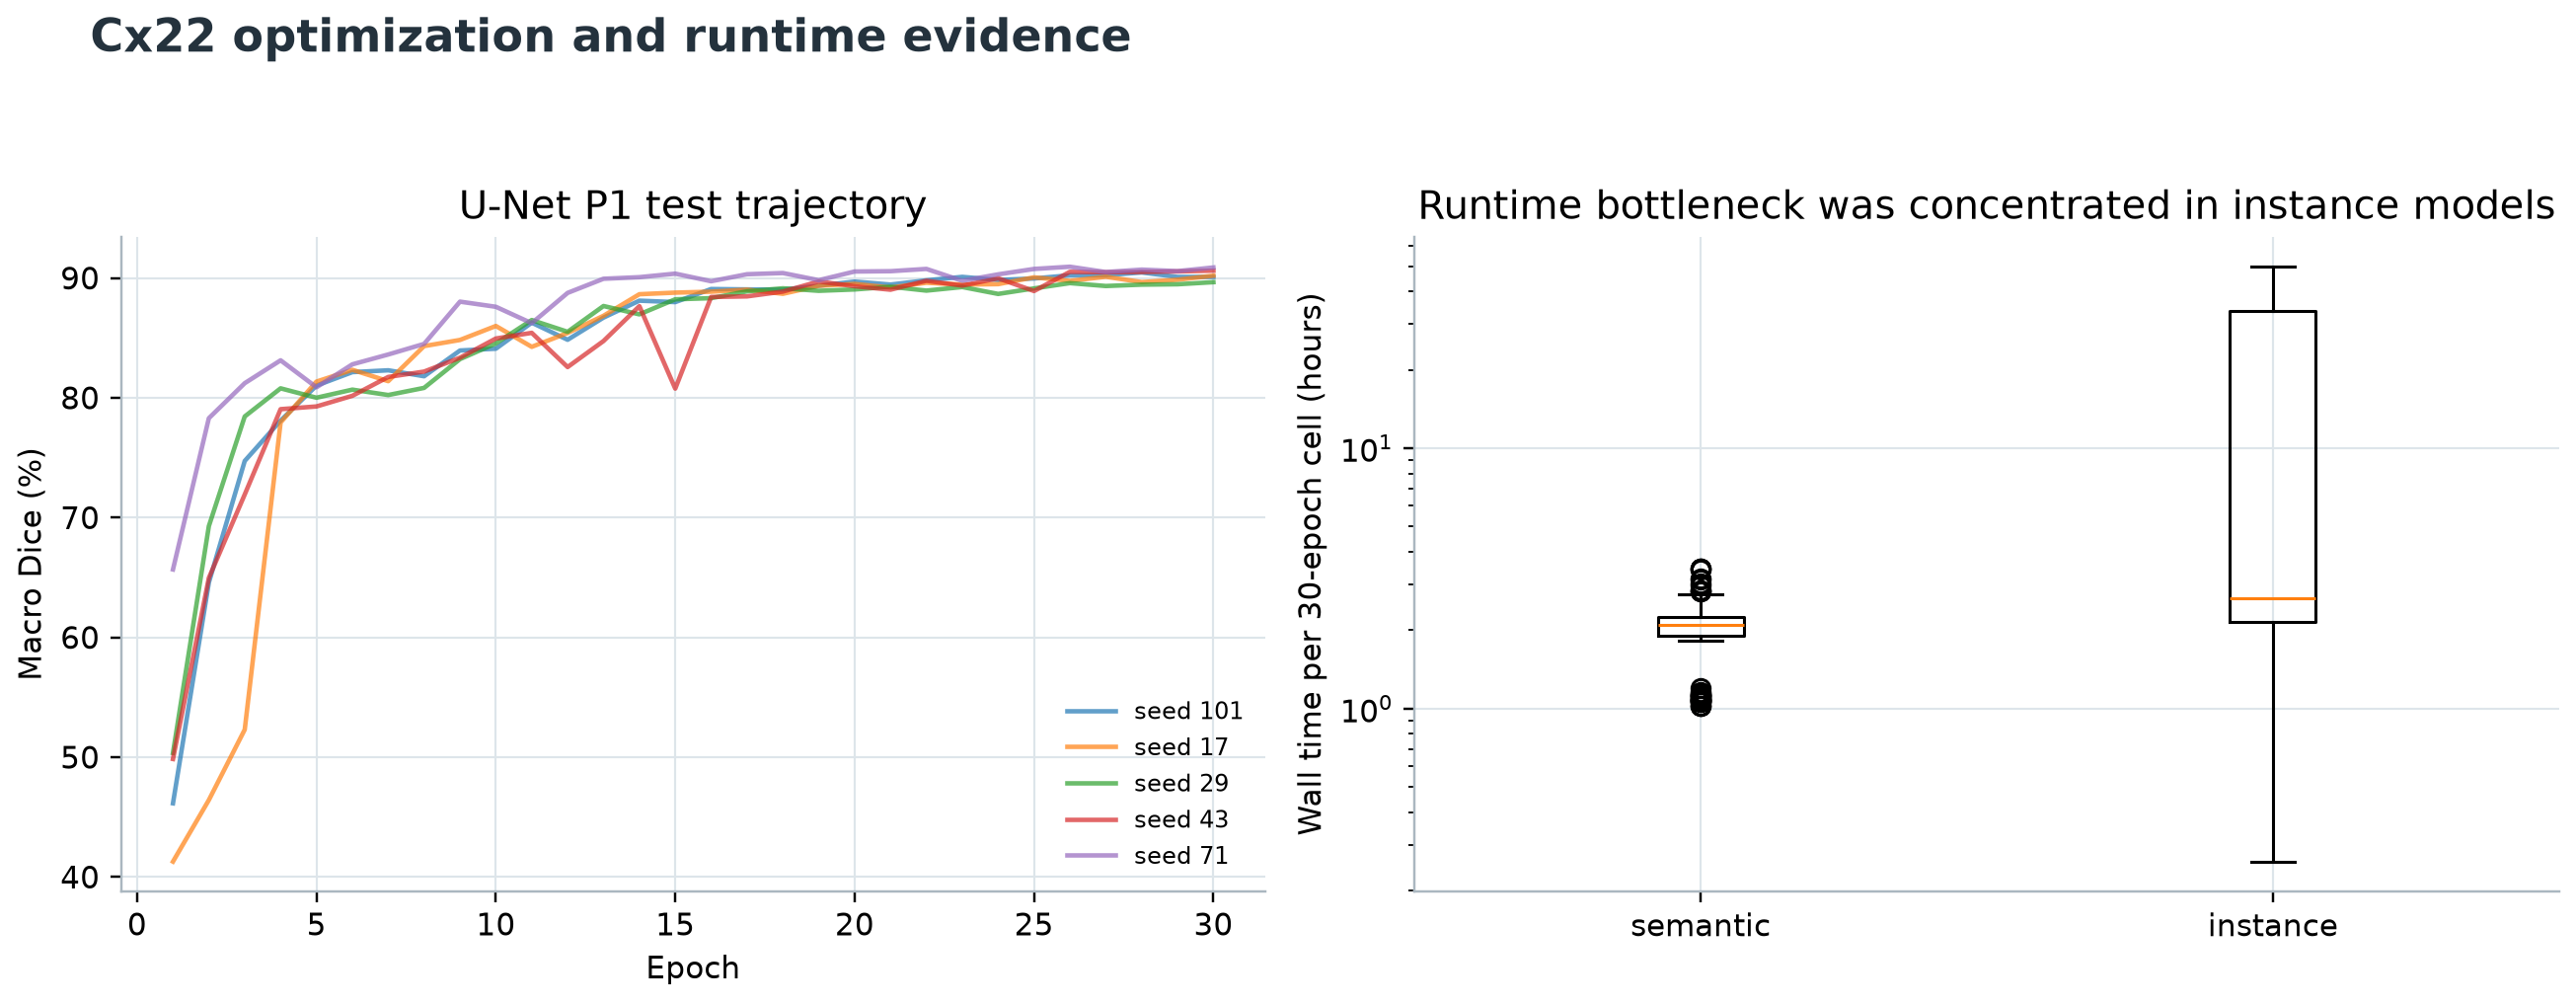
\includegraphics[width=\textwidth]{cx22_training_runtime.png}
\caption{Cx22 run-time distribution. Instance segmentation dominates the computational cost and has a long tail; the plot makes the operational bottleneck explicit.}
\label{s1:fig:cx22-runtime}
\end{figure}

The 125 semantic cells consumed 253.33 summed run-hours, with median cell time 2.09 hours. The 50 instance cells consumed 646.76 summed run-hours, with median 2.64 hours and range 0.258--49.79 hours. The complete Cx22 matrix consumed 900.08 summed run-hours. Up to three jobs were concurrent, so the sum is not wall-clock project duration.

As in classification, final model weights and per-pixel predictions were not retained after the completed JSON was written. Figure~\ref{s1:fig:cx22-labels} therefore visualizes real released ground truth, not a simulated qualitative prediction. A post-hoc prediction gallery would require fresh inference and is deliberately outside the frozen record.
